
\section{Question 4}

\begin{itemize}
    \item  Define an MLP with only one hidden layer and set the hidden layer dimension as 50. Train
    the MLP to reconstruct input images from all 10 digits
    \item  Report the Mean Squared Error on the training, validation and test set. Report your hyper-
    parameter details.
    \item Pick 5 images for each digit from the test set. Visualize the original images and the reconstructed images using the MLP.
   
\end{itemize}

\begin{solve}

\subsection{Model for Reconstruction}

\begin{lstlisting}[language=python]
RegressionMLP(
  (fc1): Linear(in_features=784, out_features=50, bias=True)
  (activation): ReLU()
  (fc2): Linear(in_features=50, out_features=784, bias=True)
  (activation_output): Tanh()
)
criterion = nn.MSELoss()
optimizer = torch.optim.Adam(model.parameters(), lr=1e-3)
\end{lstlisting}

%%%%%%%%%%%%%%%%%%%%%%%%%%%%%%%%%%%%%%%%%%%%%%%%%%%%

\subsection{Reporting Train, Val, and Test MSE Loss }

\begin{itemize}
    \item Train Loss:
   \\ Epoch 1, Loss: 0.0991
   \\ Epoch 2, Loss: 0.0804
   \\ Epoch 3, Loss: 0.0737
   \\ Epoch 4, Loss: 0.0771
   \\ Epoch 5, Loss: 0.0730
   \\ Epoch 6, Loss: 0.0712
   \\ Epoch 7, Loss: 0.0752
   \\ Epoch 8, Loss: 0.0686
   \\ Epoch 9, Loss: 0.0668
   \\ Epoch 10, Loss: 0.0684
   \\ Epoch 11, Loss: 0.0681
   \\ Epoch 12, Loss: 0.0696
   \\ Epoch 13, Loss: 0.0711
   \\ Epoch 14, Loss: 0.0697
   \\ Epoch 15, Loss: 0.0751
   \\ Epoch 16, Loss: 0.0754
   \\ \hl{Epoch 17, Loss: 0.0641}
   \\ Epoch 18, Loss: 0.0672
   \\ Epoch 19, Loss: 0.0669
   \\ Epoch 20, Loss: 0.0687
    \item Validation Loss:  0.07
    \item Test Loss:  0.07
\end{itemize}

\subsection{Reconstructed Images vs Original Images for Digits 0 to 9}
%%%%%%%%%%%%%%%%%%
\begin{figure}[H]
\centering

\begin{subfigure}{.5\textwidth}
  \centering
  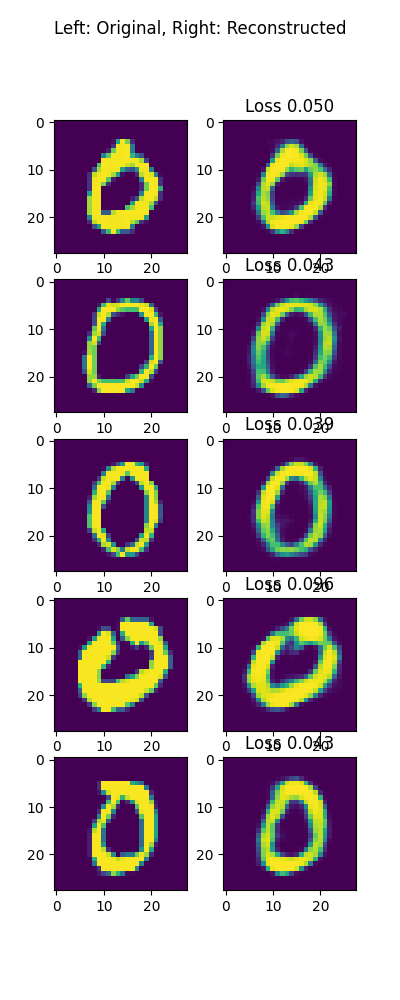
\includegraphics[width=.9\linewidth]{plots/output_0.png}
%   \caption{Left:}
\end{subfigure}%
\begin{subfigure}{.5\textwidth}
  \centering
  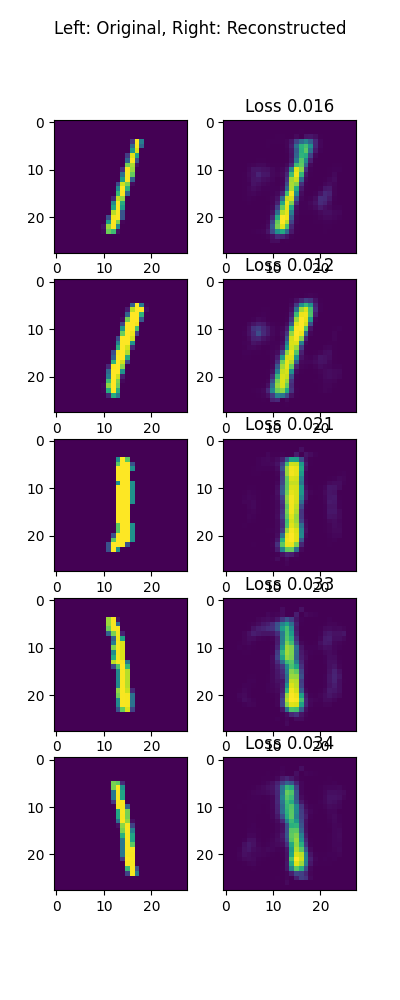
\includegraphics[width=.9\linewidth]{plots/output_1.png}
%   \caption{A subfigure}
\end{subfigure}
\end{figure}
%%%%%%%%%%%%%%%%%%
\begin{figure}[H]
\begin{subfigure}{.5\textwidth}
    \centering
    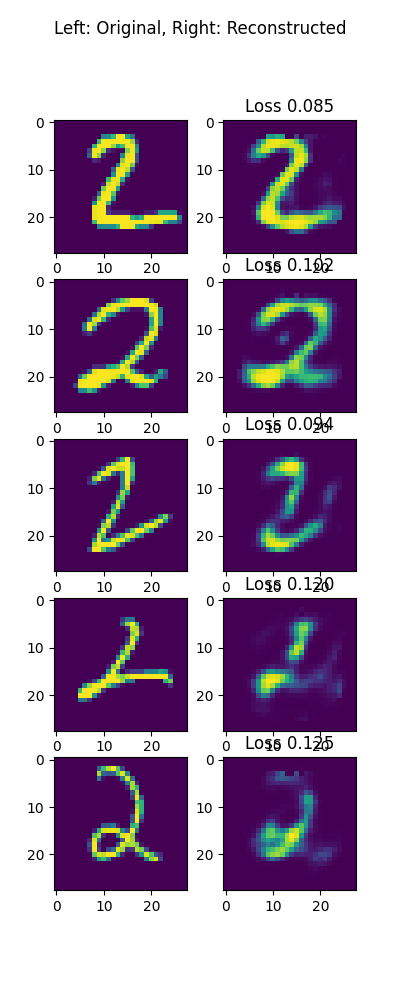
\includegraphics[width=.9\linewidth]{plots/output_2.png}
    % \caption{A subfigure}
  \end{subfigure}%
  \begin{subfigure}{.5\textwidth}
    \centering
    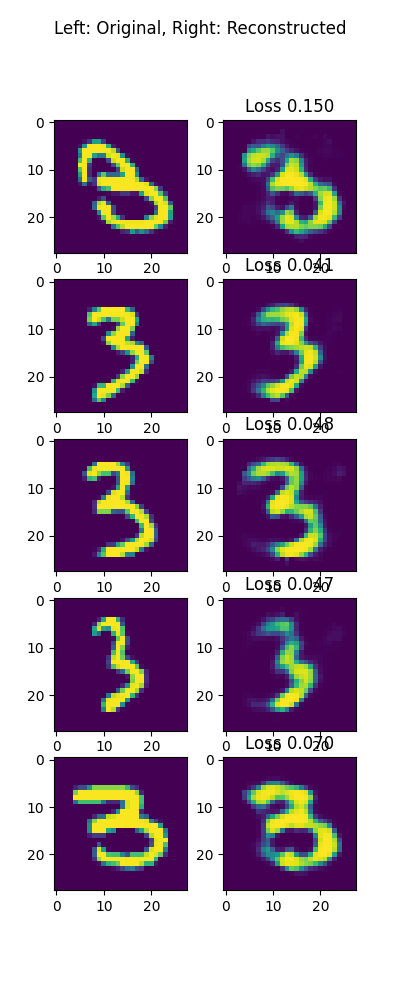
\includegraphics[width=.9\linewidth]{plots/output_3.png}
    % \caption{A subfigure}
  \end{subfigure}
  \end{figure}
%%%%%%%%%%%%%%%%%%

%%%%%%%%%%%%%%%%%%
\begin{figure}[H]
    \centering
    
    \begin{subfigure}{.5\textwidth}
      \centering
      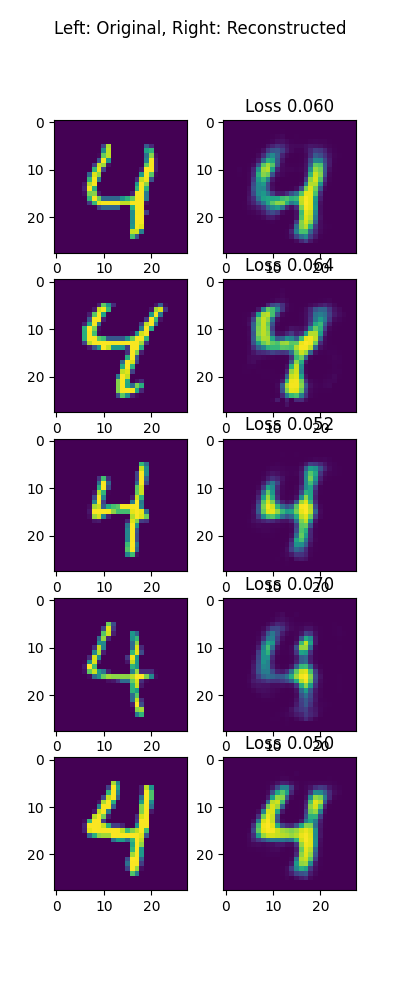
\includegraphics[width=.9\linewidth]{plots/output_4.png}
    %   \caption{Left:}
    \end{subfigure}%
    \begin{subfigure}{.5\textwidth}
      \centering
      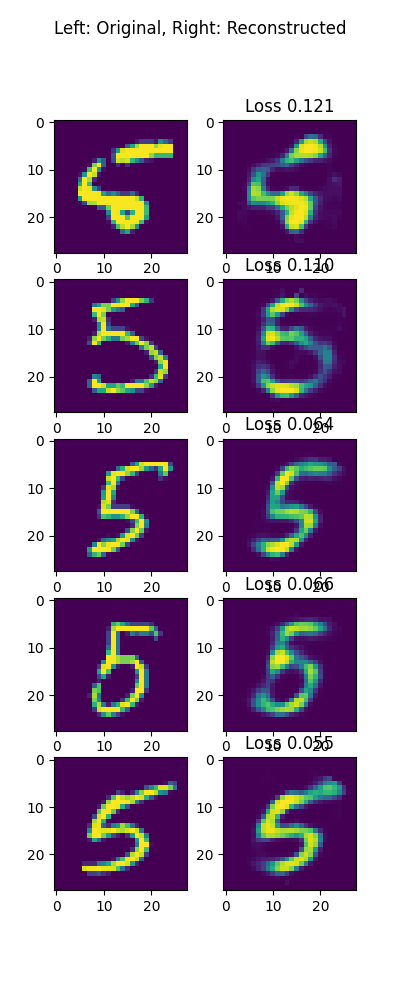
\includegraphics[width=.9\linewidth]{plots/output_5.png}
    %   \caption{A subfigure}
    \end{subfigure}
    \end{figure}
    %%%%%%%%%%%%%%%%%%
    \begin{figure}[H]
    \begin{subfigure}{.5\textwidth}
        \centering
        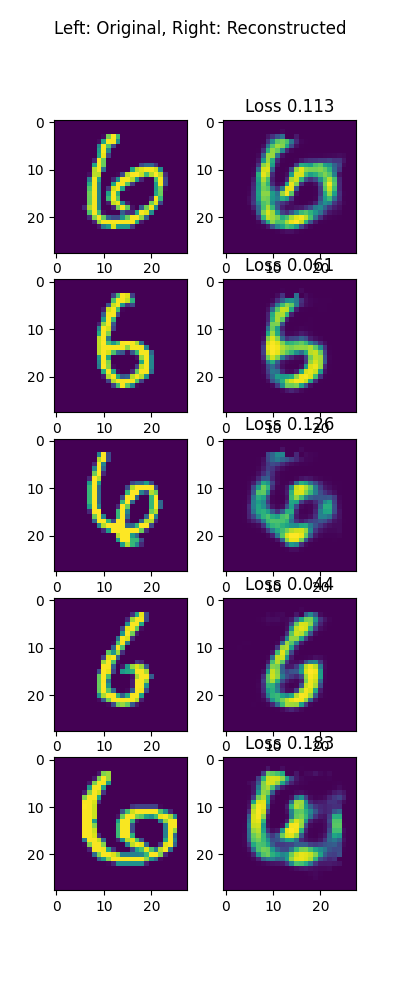
\includegraphics[width=.9\linewidth]{plots/output_6.png}
        % \caption{A subfigure}
      \end{subfigure}%
      \begin{subfigure}{.5\textwidth}
        \centering
        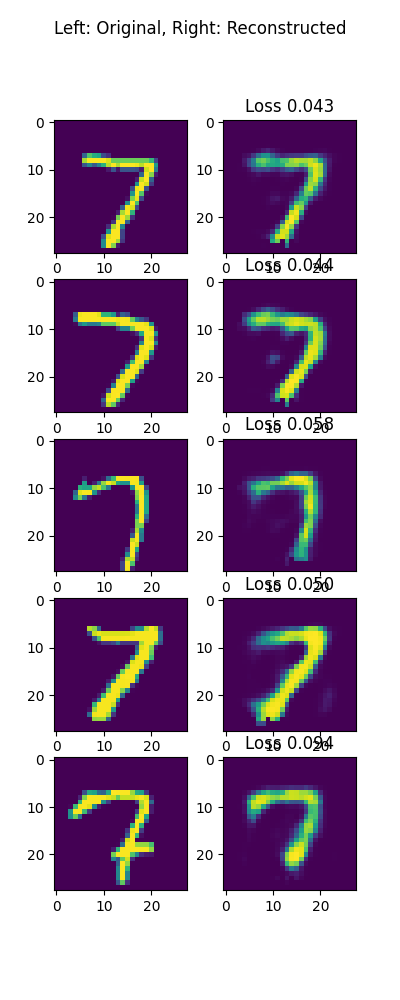
\includegraphics[width=.9\linewidth]{plots/output_7.png}
        % \caption{A subfigure}
      \end{subfigure}
      \end{figure}
    %%%%%%%%%%%%%%%%%%
        %%%%%%%%%%%%%%%%%%
        \begin{figure}[H]
            \begin{subfigure}{.5\textwidth}
                \centering
                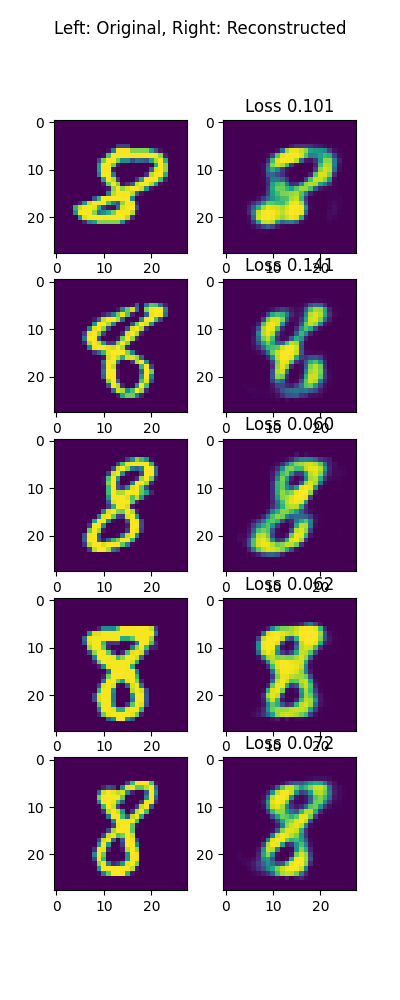
\includegraphics[width=.9\linewidth]{plots/output_8.png}
                % \caption{A subfigure}
              \end{subfigure}%
              \begin{subfigure}{.5\textwidth}
                \centering
                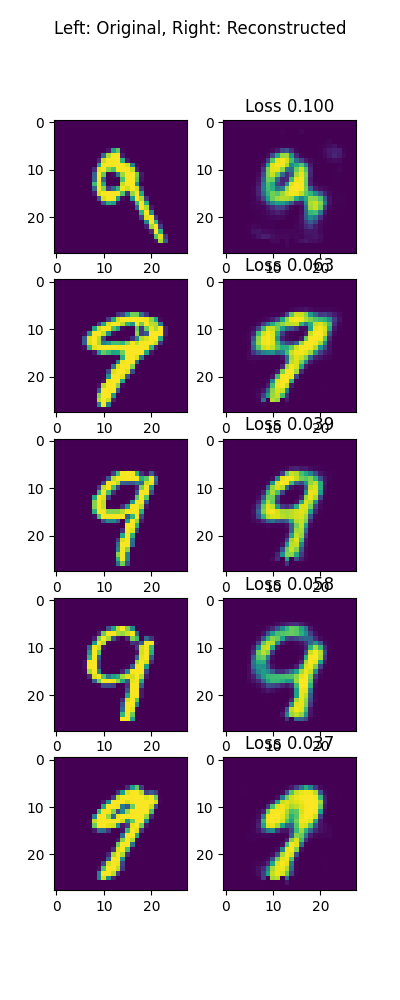
\includegraphics[width=.9\linewidth]{plots/output_9.png}
                % \caption{A subfigure}
              \end{subfigure}
              \end{figure}
            %%%%%%%%%%%%%%%%%%
            
\end{solve}